\clearpage

\def\chaptertitle{Methodology}

\lhead{\emph{\chaptertitle}}

\chapter{\chaptertitle}
\label{ch:methodology}

Based on the overview of and challenges faced by edge computing paradigms in conforming to SLA constraints, the stated research questions, and the related works discussed above, a hybrid auto-scaling algorithm to answer these questions was proposed during the course of this research project.\par

In this chapter, a brief discussion surrounding the problems and challenges of auto-scaling edge architecture deployments in an SLA-compliant manner will be conducted in section \ref{sec:ch3-problem-overview}. Section \ref{sec:ch3-hybrid-autoscale-overview} will detail the high-level overview of the proposed hybrid autoscaler, the objectives of the algorithm, and the challenges it faces.

\section{Problem Overview}
\label{sec:ch3-problem-overview}

Edge architectures are split into three layers \cite{hamdan2020edge}. 
The cloud layer complements cloud-computing paradigms, wherein it manages the entire network architecture. The edge layer consists of data storage and communication with user devices. Finally, the device layer consists of all the user devices that will interact with the edge architecture.\par

\begin{figure}[htb]
    \centering
    \caption{Autoscaling problem overview}
    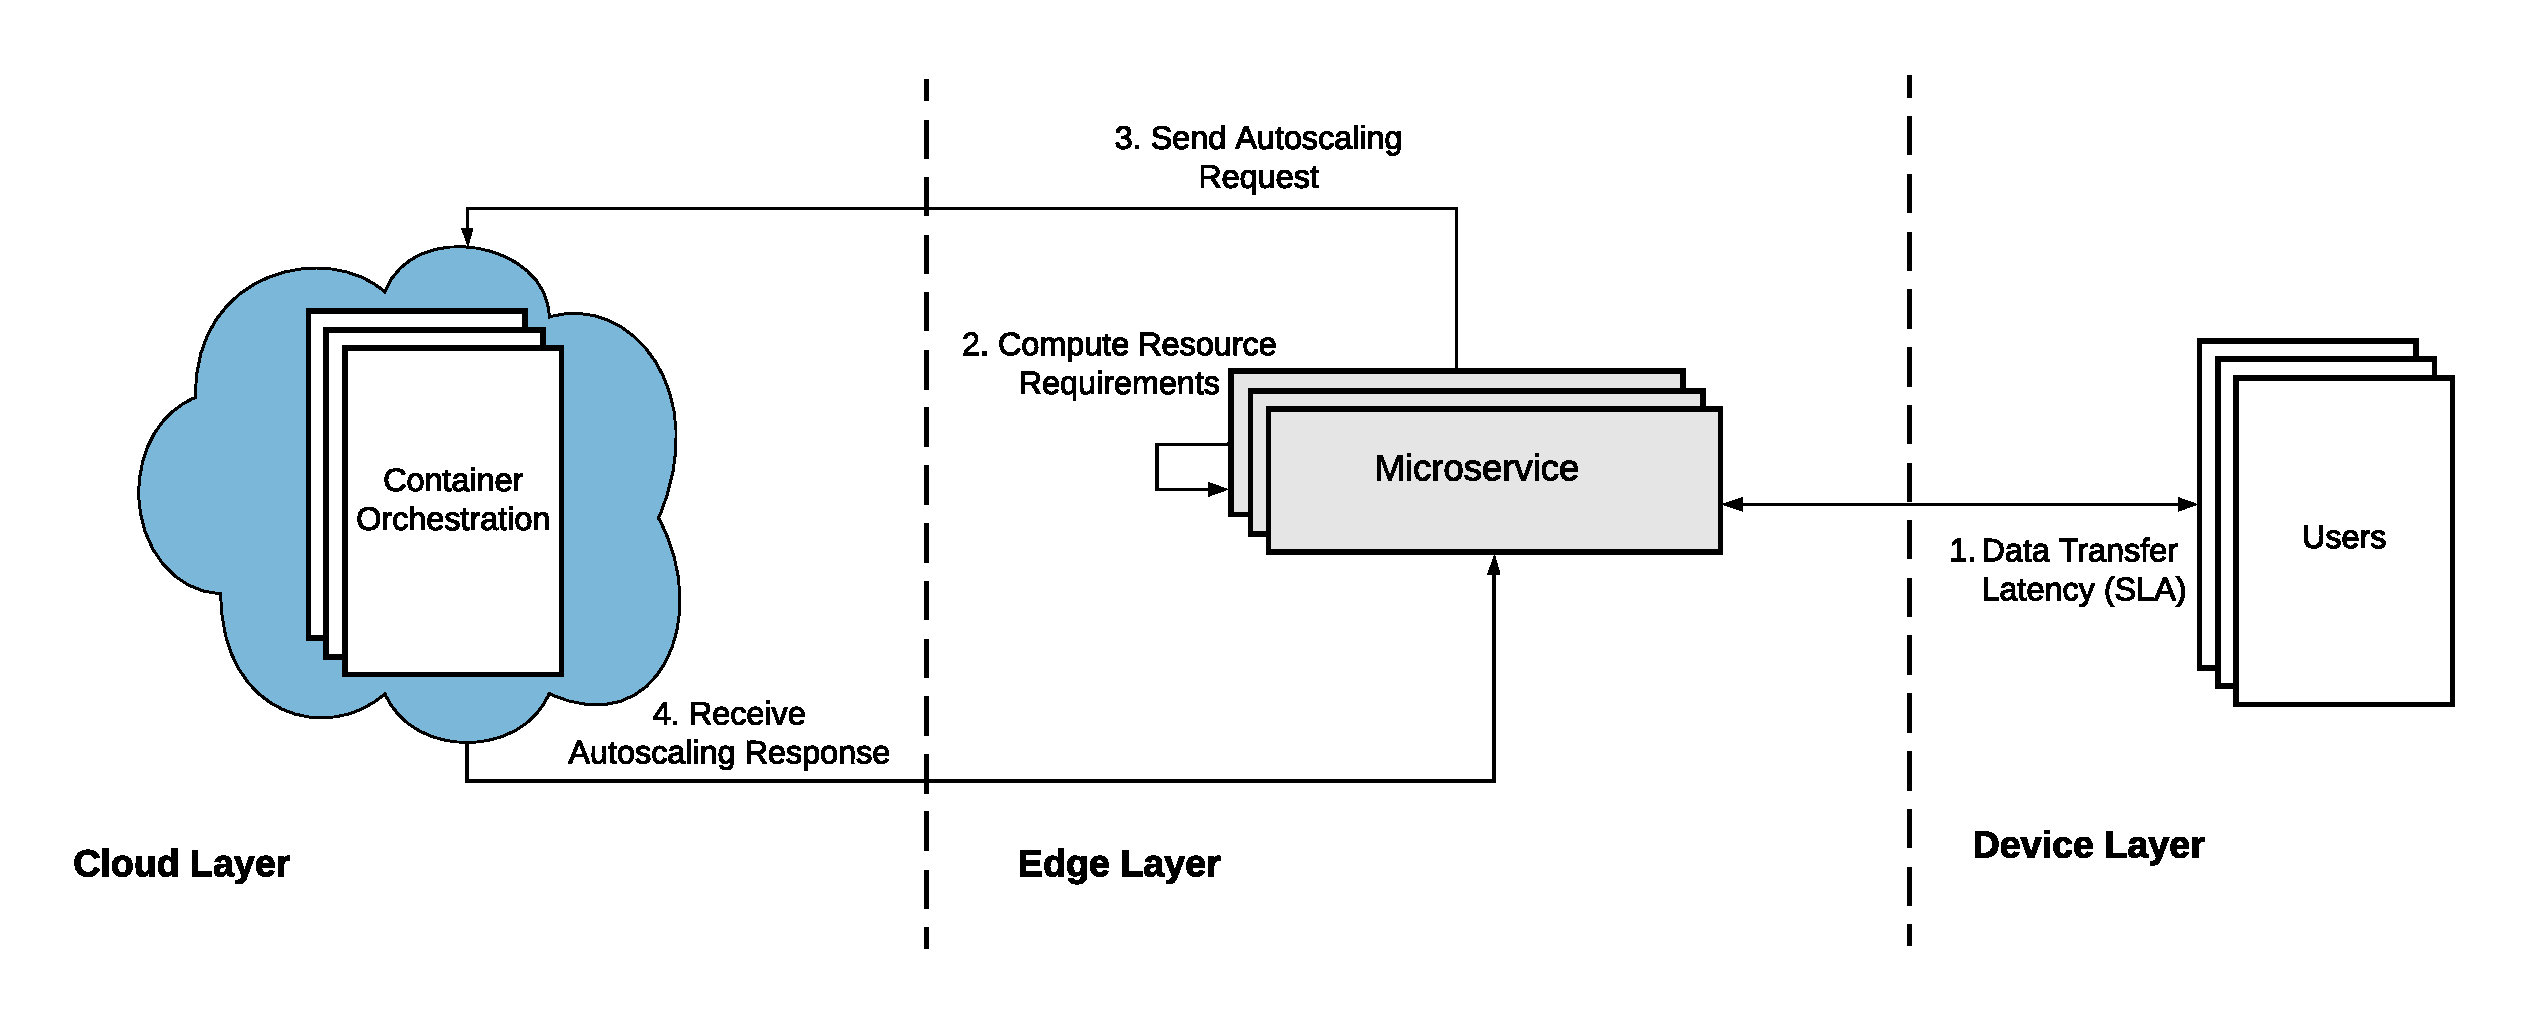
\includegraphics[width=0.8\linewidth]{Figures/Problem-Overview.pdf}
    \label{fig:autoscaling-problem-overview}
\end{figure}

The cloud layer has the most amount of resources allocated to it, as it is in charge of managing the entire network, and coordinating the resource allocation of the edge layer. However, the primary drawback is the distance between the user and the cloud layer which results in significant latency, making it unsuitable for serving real-time user requests. Thus only system critical applications such as the micro-service control plane are deployed on this plane. The edge layer has far fewer resources than the cloud layer, but its proximity to the users results in lower network latency, making it ideal for resources scaling. For this reason, the edge layer consists of the micro-service worker nodes. These nodes allocate resources dynamically according to user requirements through the process known as auto-scaling.\par

Figure \ref{fig:autoscaling-problem-overview} shows the auto-scaling process. The users in the device layer send requests and receive responses to the micro-service deployment in the edge layer. The time taken to receive this response is considered to be the SLA latency metric negotiated between the edge deployment provider and the customer. Using the number of requests being received by the user layer, the edge layer micro-service autoscaler computes the total resource requirements to serve the customer. Based on its findings, the edge layer requests the container orchestration in the cloud layer to either downscale or upscale its resources. The container orchestrator then computes the resource allocation location, and sends its response back to the edge layer.\par

%TC:ignore
\begin{table}
    \caption{Definition of Symbols}\label{tab:lstm-params}
    \centering
    \begin{tabular}{|l l|}
        \hline
        Symbol & Definition\\
        \hline
        $\mathcal{S}_{v}(t)$ & The value of the SLA metric at time $t$\\
        $\Delta$ & Maximum SLA metric threshold agreed by cloud provider and customer\\
        $\mathcal{C}_{t}$ & ``Cold start'' time taken to scale resource replicas\\
        $req_{RT}(t)$ & Round trip latency of user request to edge layer\\
        $\mathcal{K}_{t}$ & Constant latency present between edge and device layers\\
        $\mathcal{U}(t)$ & Latency of deployment with unitary resource replica\\
        $\mathcal{D}$ & Total resources in micro-service deployment\\
        $p_{i}$ & Resource pod $i$ of deployment $\mathcal{D}$ where $i = \{1, 2, .. N\}$\\
        \hline
    \end{tabular}
\end{table}
%TC:endignore

For real-time applications, the auto-scaling should adhere to SLA metric as much as possible, and try to minimize the number of violations. The SLA metric violation $\mathcal{S}_{v}(t)$ is defined as when it exceeds a certain threshold $\Delta$ agreed by both the cloud provider and the customer.
\begin{equation}
    \mathcal{S}_{v}(t) > \Delta
\end{equation}

The threshold $\Delta$ is typically split into three categories:
\begin{itemize}
    \item Flexible - This is typically the highest allowed violation threshold for the application. Flexible SLA metrics are used to gauge the availability of the deployment. Most IoT applications employ this threshold.
    \item Strict - This is the lowest allowed violation threshold in the application. This threshold is significantly challenging to maintain, and is used by extremely time-critical applications such as remote tools for surgery.
    \item Moderate - This threshold is a trade-off between flexible and strict SLA thresholds. This threshold is used by applications to ensure a real-time capability such as traffic light scheduling in railways.
\end{itemize}

The auto-scaling will thus use a resource metric to scale its resources up or down. The autoscaler will check to see if the micro-service metric exceeds the threshold for a certain time period, and if so, autoscale resources accordingly. A problem arises in the time it takes to scale these resources, however. This time to increase the number of resource replicas $\mathcal{R}$, known as cold start $\mathcal{C}(t)$ can be written as:

\begin{equation}
    \mathcal{C}(t) = \mathcal{R}_{download}(t) + \mathcal{R}_{deploy}(t) + \mathcal{R}_{register}(t)
\end{equation}

The replica download time is usually a one-time delay due to optimizations done on modern container orchestration software, and can be ignored for SLA latency calculations. Thus, we can reduce this equation to the following:

\begin{equation}
    \mathcal{C}(t) \approx \mathcal{R}_{deploy}(t) + \mathcal{R}_{register}(t)
\end{equation}


This time to deploy and register the replica to the container orchestration tool cannot be avoided. Furthermore, it can be shown that the number of SLA violations $\mathcal{V} \propto \mathcal{C}(t)$ due to the correlation between cold-start delay and the lack of available resources.\par

Thus, when computing the SLA violation for a latency metric, the SLA latency can be re-written as the sum of the cold-start time and the round-trip time taken for the request.

\begin{equation}
    \mathcal{S}_{v}(t) = \mathcal{C}(t) + req_{RT}(t)
\end{equation}


This round-trip time is the combined sum of the inherent delay present in the network layer, and the time taken for the edge application to process the request.

\begin{equation}
    req_{RT}(t) = 2 \times latency_{N/W} + latency_{app}
\end{equation}

The network delay can be reduced by investing in higher network bandwidths, but such improvements are out of scope of the project. Here we consider this latency to be a constant $\mathcal{K}$. Furthermore, $latency_{app}$ is inversely proportional to the available resources to the application. Using this information, $req_{RT}(t)$ is approximated as:

\begin{equation}
    req_{RT}(t) \approx \mathcal{K}(t) + \frac{\mathcal{U}(t)}{resources_{app}}
\end{equation}

Where $\mathcal{U}(t)$ is the app latency of a deployment with a unitary resource deployment. For horizontal pod autoscaling, the resources here are the number of pods in deployment $\mathcal{D}$ such that $\mathcal{D} = \sum_{i} p_{i}$, where $i$ represents the current number of deployed pods. These pods process the request. The final SLA equation can be re-written as follows:

\begin{equation}
    \mathcal{S}_{v}(t) = \mathcal{C}(t) + \frac{\mathcal{U}(t)}{\sum_{i} p_{i}} + \mathcal{K}(t)
\end{equation}

Thus, the primary aim of the proactive autoscaler is to significantly reduce or even eliminate the cold start, while the reactive autoscaler aims to increase the number of resources assigned to the deployment to minimize the application latency.\par

From the above equation, it is clear that as $\sum_{i} p_{i}$ approaches $\infty$, the value of $\frac{\mathcal{U}(t)}{\sum_{i} p_{i}}$ approaches 0. Thus, why not simply allocate the maximum number of pods to the deployment?\par

Most cloud providers allocate a cost $\mathcal{L}$ per each resource assignment to the deployment. If the maximum number of pods which can be deployed is $N$, the cost is calculated as follows.

\begin{equation}
    cost = \alpha \times \sum_{i} p_{i} \quad ;\,i \le N
\end{equation}

Where $\alpha$ is the unitary resource cost which may vary depending on the resource provider. Thus, simply scaling all resources to the maximum amount may result in significant and infeasibly high deployment costs. Thus the auto-scaling equation can be converted to an optimization problem. The objective of the autoscaler is to maximize resources in a way which minimizes both the latency, as well as the cost. Furthermore, the customer will have a maximum cost $\mathcal{L}$ which the deployment must not exceed. Determining whether or not the resource allocation of at least $\mathcal{D}$ without exceeding this cost $\mathcal{L}$ is possible, is akin to the famous Knapsack decision problem \cite{kellerer2004introduction}. This decision problem is NP-Complete, and as such no known algorithm can compute this auto-scaling decision in polynomial time \cite{martello1987algorithms}. Due to this drawback, most autoscalers rely on a reactive rule-based or proactive machine learning technique to compute a close approximation.\par

A problem arises, however, in the amount of time and resources it takes to train a proactive model. Not only is a significant amount of CPU and memory resources consumed in the training process, but a large time-series data set is also required to generate sufficient number of training windows, without which the model will provide erroneous results until such time as the model is adequately trained. While hybrid models help to mitigate the initial errors via the reactive auto-scaling component, the questions regarding the model complexity remained an open issue.\par

Another issue in proactive autoscalers is that not only does it predict increases in utilization before-hand, it also does so for the drop-off in utilization. This can lead to the edge deployment prematurely reducing its resources due to the drop-off forecast, causing several SLA violations due to low availability of resources. To offset this, several hybrid algorithms combine the readings of their reactive and proactive autoscalers, and autoscale according to the highest reading. While this approach works, such algorithms render the accurate resource drop-off predictions of the forecaster redundant, merely taking up precious computation space in the edge deployment.\par

In most proactive autoscalers, the forecaster attempts to perfectly model the time-series curve to assign resources. Even in the hybrid algorithms that have been proposed in chapter \ref{ch:background}, the proactive sections of the autoscalers are generally unmodified proactive forecasters bundled together with a reactive component. This strategy of attempting to perfectly forecasting the curve is what takes such large amounts of resources.\par

In the autoscaler proposed in this thesis, the autoscaler will not attempt to predict the exact resource workload. Instead, the time-series graph is heavily simplified using a noise filtering method, and then inputted to the machine learning model. Furthermore, the LSTM only attempts to forecast the exact times when resource requirements starts to increase. Every other requirement, such as the stable resource utilization, as well as the drop-off in non-peak time periods can be handled by the reactive autoscaler, thus heavily simplifying the forecaster architecture. The simplified forecaster has an additional benefit in not requiring incredibly lengthy amounts of time-series data to be stored for it to make accurate predictions, thus this data can also be kept in the edge layer. This makes the autoscaler extremely lightweight and responsive, and thus capable of being deployed in an edge environment.\par

\section{Proposed Hybrid Autoscaler}
\label{sec:ch3-hybrid-autoscale-overview} 

\begin{figure}[htb]
    \centering
    \caption{Proposed hybrid architecture overview}
    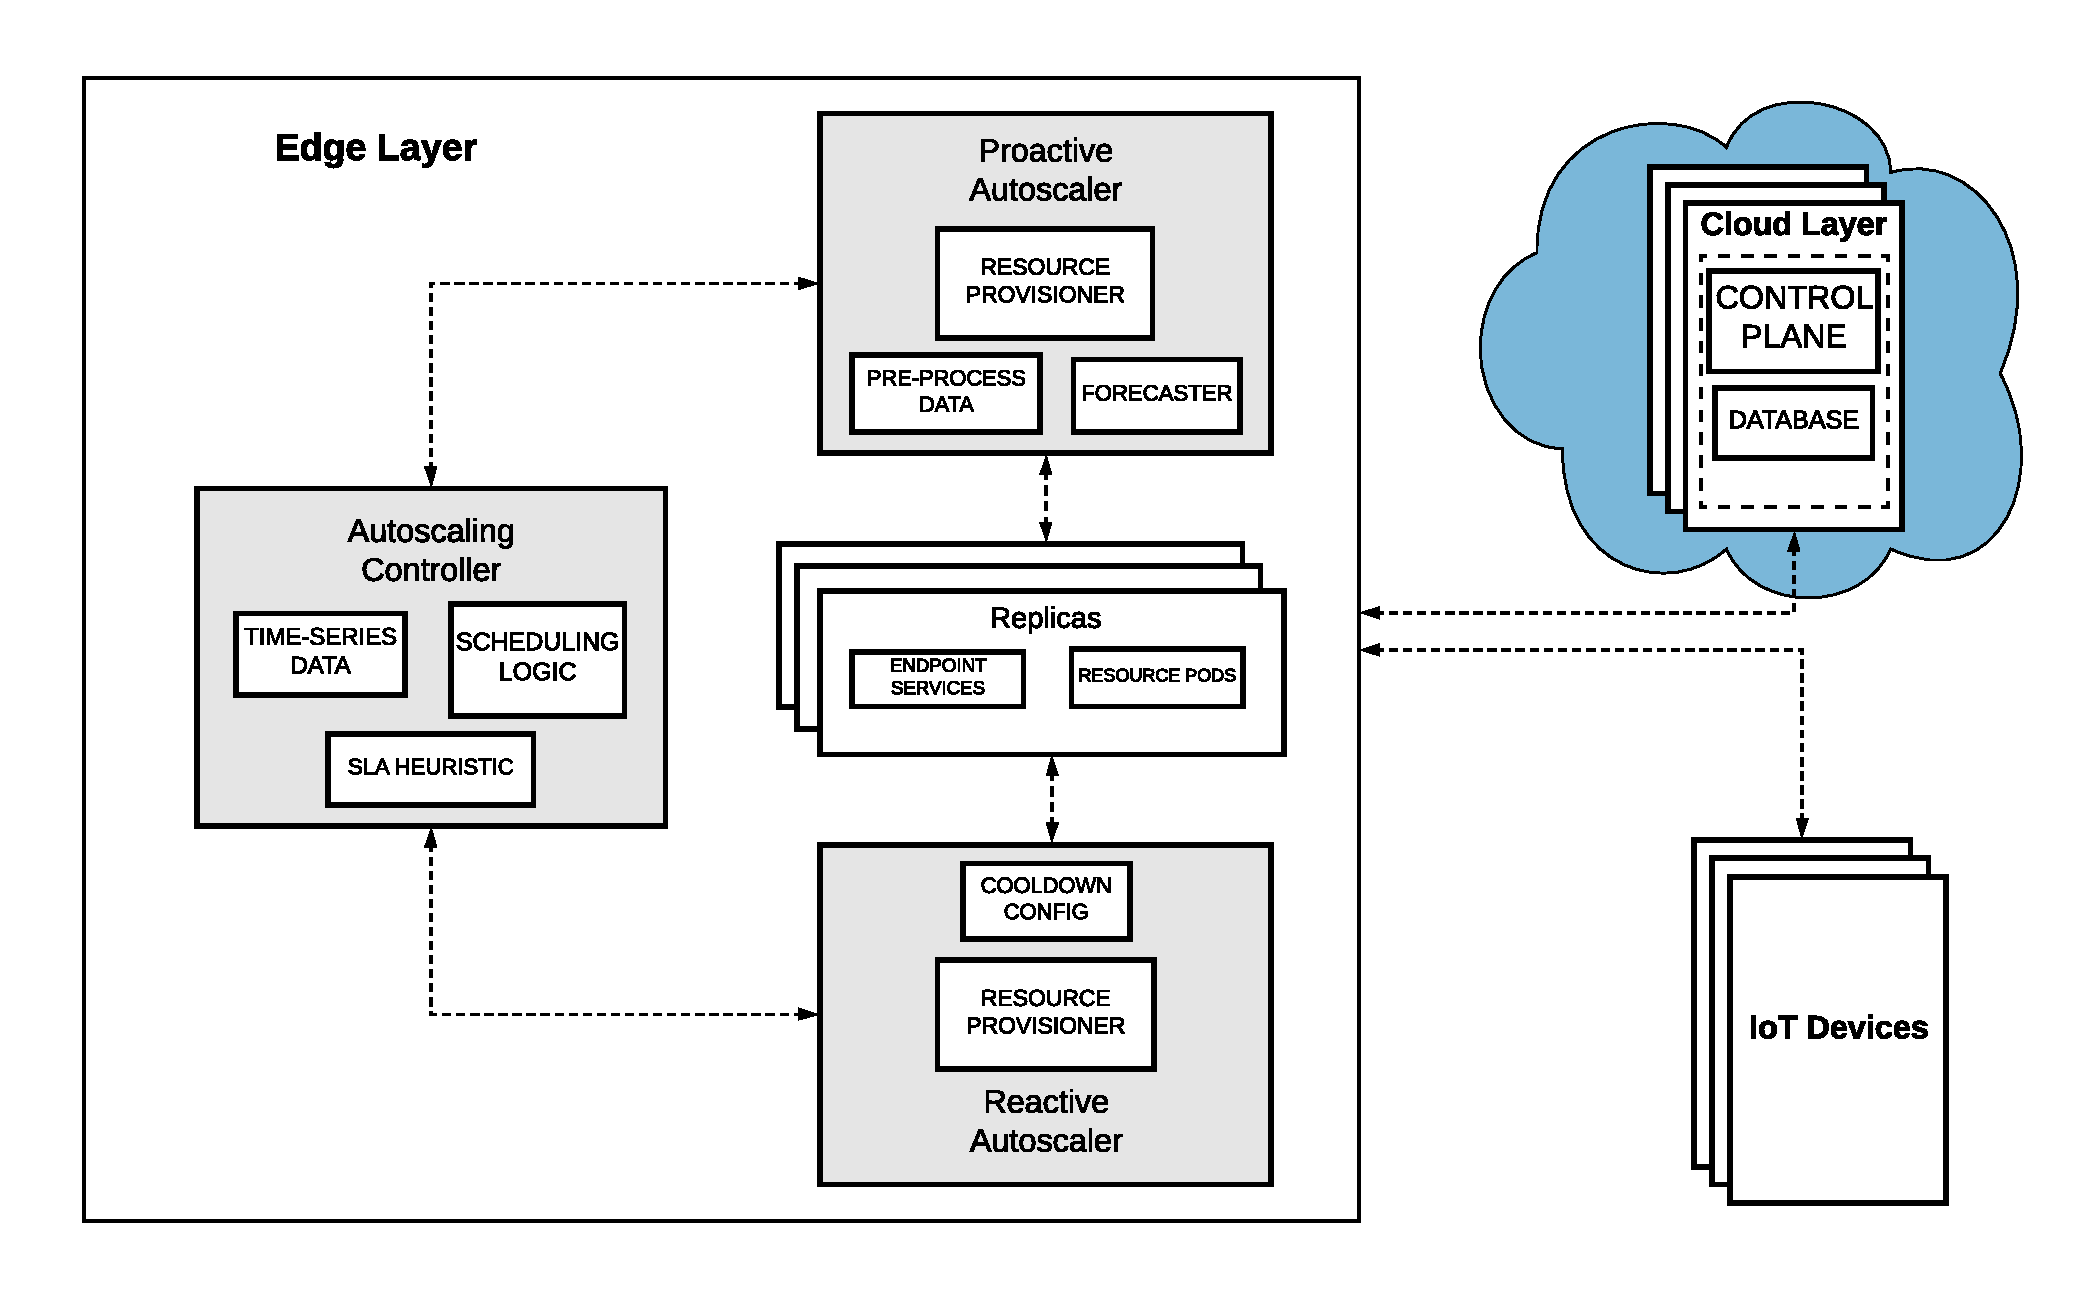
\includegraphics[width=1.0\linewidth]{Figures/Hybrid-Architecture-Overview.pdf}
    \label{fig:hybrid-arch-overview}
\end{figure}

An overview of the hybrid autoscaler architecture is shown in figure \ref{fig:hybrid-arch-overview}. The edge node consists of three main sections. The first is the reactive autoscaling subsystem, which has the resource provisioner, and the configuration which dictates the cool-down logic for scaling up and down. As Zhang et al. \cite{zhang2019quantifying} demonstrated, the microservice system stability is directly related to the careful selection of cooldown parameters. Thus, these must be available to the user in a configuration setting.\par

\suhrid{TODO: Make sure to discuss the proactive autoscaler in detail in Ch3 using the notes written in Ch2 \cmark}
The second subsystem is the proactive autoscaler. From a high-level perspective there are three main components. The resource provisioner is similar to that of the reactive autoscaler, however it also consists of a forecaster using machine learning techniques, and a data pre-processing algorithm. This algorithm removes any noise present in the time series data, and smoothens the graph, making it easier for the forecaster to make predictions in a low-cost manner. A detailed explanation of the forecaster logic itself will be discussed in chapter \ref{ch:experimental-setup}.\par

Finally, the auto-scaling daemon controls which auto-scaling logic will be applied to the replicas, and also keeps a track of any SLA violations. It also hosts the time-series metric data, and has a feedback loop with the proactive autoscaler. If it detects any SLA violations caused after autoscaling during a configured time window, it automatically adjusts the hyper-parameters of the proactive forecaster in an attempt to predict the time-series in a more accurate manner during the next training iteration. Correspondingly, a lack of SLA violations during a specific time period reverts the autoscaler parameters to attempt to streamline the training process further. Such a heuristic method allows for the freeing up of the complex hyper-parameter tuning process seen in most proactive models. This is a key part of the architecture which is essential in answering one of the research questions outlined in the thesis.\par

\suhrid{In methodology, detail the reactive and proactive portions - detail only the algorithm pseudo-code \cmark}

\subsection{Architecture Overview}
\label{subsec:ch3-hybrid-arch}

At a high-level, the default Kubernetes horizontal pod autoscaler operates on the ratio between the current and desired metric values, which can be written as:

\begin{equation}
    replicas_{desired} = \lceil replicas_{current} \times \frac{metric_{current}}{metric_{desired}}\rceil
\end{equation}

For example, for a given deployment with current replica count as 1, if the desired metric value is 50 resource units, the current value is 100, then the number of desired replicas will be $\lceil 1 \times \frac{100}{50}\rceil = 2$. There are three other important parameters which are key to controlling the process of horizontal pod scaling, namely ``tolerance'', ``scale up cooldown'', and ``scaledown cooldown''.\par

The tolerance is a constant which informs the Kubernetes autoscaler when to skip calculating new replicas. The tolerance ratio, can be calculated as:

\begin{equation}
    \label{eqn:tolerance}
    tolerance = \abs{ \frac{metric_{desired} - metric_{current}}{metric_{desired}} }
\end{equation}

For example, if the current metric is 60, and the desired metric is 50, the tolerance is calculated as $ tolerance = \abs{ \frac{60 - 50}{60}} = 0.167$. By default, if the tolerance value is below 0.1, autoscaling is skipped for that control loop, however this can be configured by the user.\par

The scale up and scale down cooldowns control how quickly autoscaling occurs. The default approach which is set by Kubernetes can be concisely stated as ``Scale up as quickly as possible, while scale down very gradually''. Therefore, the default scale up cooldown is set to 0 seconds, meaning that the moment the desired replica value increases, the autoscaling will be initiated. However, the default cooldown is set to 300 seconds, meaning that if the desired replica value is decreased, it must remain decreased for 300 seconds (or 20 control loops) before the resources are scaled down.\par

A cooldown value which is too low would cause a repetitive upscaling and downscaling of the resources, leading to a significant stress on the system as well as a wastage of resources. Meanwhile, a large value would render the autoscaler unable to assign resources quickly enough to ensure SLA latency compliance. Thus, for the proposed autoscaler, a moderate cooldown value was chosen to ensure best system stabilty and SLA compliance. This cooldown configuration would be applied to both the proactive and reactive auto-scaling sub-components.\par

For auto-scaling proactively, a custom metric $metric_{forecast}$ is used, which defines the future CPU workload expected to be exerted on the social media application $\mathcal{T}$ seconds in the future, where $\mathcal{T}$ can be configured by the user. This $metric_{forecast}$ value will be sent to the auto-scaling daemon by the proactive autoscaler.\par

The autoscaler daemon consists of a scheduling logic controller which handles how to switch between proactive and reactive auto-scaling. Algorithm \ref{alg:scheduling-logic-daemon} explains how the hybrid scheduling logic determines which auto-scaling subsystem to employ. The hybrid scheduler takes four inputs, namely the $replicas_{current}$, $metric_{current}$, $metric_{desired}$, and $metric_{forecast}$ variables discussed above. It outputs one value, the $replicas_{desired}$.\par

The autoscaler computes two replica values, one for the proactive forecaster which determines the replicas after $\mathcal{T}$ seconds, and one for the reactive forecaster, which determines the current resource requirements. If it is found that the future requirements are higher than the current resource utilization, then the hybrid scheduler outputs the forecaster replica count as the desired replicas. Otherwise, the hybrid scheduler determines that the utilization is either stabilizing or about to decline. Due to this, it makes a decision that the reactive replica count is the desired number. The hybrid scheduler then sends this value to the container orchestration controller plane to autoscale the replicas accordingly using either the reactive or proactive sub-system's resource provisioner.\par

%TC:ignore
\begin{algorithm}
    \caption{Scheduling logic of the autoscaler daemon}
    \label{alg:scheduling-logic-daemon}
    \textbf{Input}: $replicas_{current},\, metric_{current},\, metric_{desired},\, metric_{forecast}$\\
    \textbf{Output}: $replicas_{desired}$
    \begin{algorithmic}
        \State $replicas_{forecast} \gets \lceil replicas_{current} \times \frac{metric_{forecast}}{metric_{desired}}\rceil$
        \State $replicas_{reactive} \gets \lceil replicas_{current} \times \frac{metric_{current}}{metric_{desired}}\rceil$
        \If{$replicas_{forecast} > replicas_{reactive}$}
            \State $replicas_{desired} \gets replicas_{forecast}$
        \Else
            \State $replicas_{desired} \gets replicas_{reactive}$
        \EndIf
        \State \Return $replicas_{desired}$
    \end{algorithmic}
\end{algorithm}
%TC:endignore

The reactive autoscaler subsystem is responsible for determining whether or not auto-scaling should proceed based on the given configuration. The reactive algorithm is built on top of the default horizontal pod autoscaler deployed by the container orchestration platform. The autoscaler is modified in such a way that it has its cooldown parameters are set to a moderate value to ensure adaptability to SLA-constrained scenarios, while also maintaining system stability. The workflow is shown below in algorithm \ref{alg:reactive-algo}. The algorithm takes the desired and current metrics as input, as well as the desired metrics, and outputs the decision to autoscale or not. It does this by computing the $tolerance$ value as shown in equation \ref{eqn:tolerance}. If this tolerance is above the configured threshold, the autoscaler will be modify the replicas, otherwise it will ignore the current auto-scaling request.\par

%TC:ignore
\begin{algorithm}
    \caption{Reactive autoscaler subsystem workflow}
    \label{alg:reactive-algo}
    \textbf{Input}: $metric_{current},\, metric_{desired}$\\
    \textbf{Output}: $autoscale$
    \begin{algorithmic}
        \State $tolerance \gets \abs{ \frac{metric_{desired} - metric_{current}}{metric_{desired}} }$
        \If{$tolerance > \gamma$}
            \State $autoscale \gets Yes$
        \Else
            \State $autoscale \gets No$
        \EndIf
        \State \Return $autoscale$
    \end{algorithmic}
\end{algorithm}
%TC:endignore

The forecaster portion of the autoscaler is used to generate this $metric_{forecast}$ value. Several time series forecaster algorithms exist, with the two prominent ones being the more modern deep learning algorithm LSTM, and the traditional deep learning algorithm ARIMA. Siami-Namini et al. \cite{siami2018comparison} demonstrated that LSTM implementations outperformed ARIMA, reducing error rates by over 80\%. Furthermore, they were able to demonstrate that the number of deep learning ``epochs'', or the total amount of training time required for LSTM did not need to be set to a high value. In fact, setting an significantly higher value than required was shown to degrade performance due to over-fitting. The authors posited that LSTM worked so well due to the ``rolling updates'' being performed on the model. The LSTM weights are only set once when the forecaster is deployed, after which they are always updated on every call of the training algorithm, meaning there is a continuous improvement to the prediction results.\par

\begin{figure}[htb]
    \centering
    \caption{Pre-processing of data, courtesy of Christopher Boucher \cite{comsolcurvefitting}}
    \label{fig:data-pre-process}
    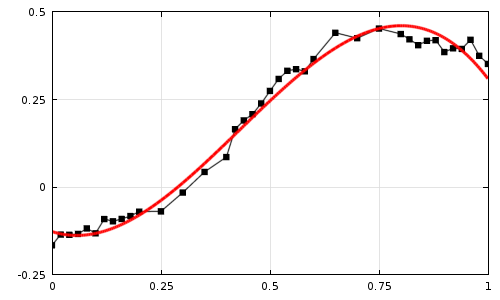
\includegraphics[width=0.6\linewidth]{Figures/Data-Pre-Processing.png}
\end{figure}

To speed up the forecast process even further and reduce the resource and time requirements, the time-series data can be pre-processed to smoothen it. Doing so makes it easier for the deep learning model to extract patterns, and reduces the training and validation loss. Figure \ref{fig:data-pre-process} shows a graph containing raw input (shown in black), and a smoothened data curve (shown in red). While the red curve contains all the requisite information of the data (such as slope of the curve, maximum and minimum value, etc.), it removes the noise, reducing the overall loss, and reducing the length of the lookback LSTM needs to perform to accurately predict future data.\par

Based on the investigations above, it was determined that LSTM time-series forecasters would be ideally suited for a proactive autoscaler designed for edge computing. Algorithm \ref{alg:proactive-forecast-alg} shows the implementation of such a forecaster. As input, the algorithm takes the variable $lookback$, which is the number of data points it should use as a window to train, $forecast$, which is the number of data points to predict, the training time $epochs$, and the $learning\_rate$, which determines the step size per each training iteration moving towards the minimum loss value. The algorithm outputs the $result$, which is an array of size $forecast$ which contains all the predicted values. The algorithm implements a control loop every $\mathcal{P}$ seconds, where it requests the latest time series data from the autoscaler daemon. It then pre-processes this data to remove the noise as shown above, and performs one iteration of training using the configured parameters. It then computes the validation loss when doing so, and accepts this model as the ideal one if it has lower validation loss than the previous iteration, otherwise rejecting the model and using the older one instead. Finally, the model predicts the future forecasts and returns them to the autoscaler daemon for later use.\par

%TC:ignore
\begin{algorithm}
    \caption{Proactive forecaster algorithm}
    \label{alg:proactive-forecast-alg}
    \textbf{Input}: $lookback \geq 0, forecast \geq 0, 0 \leq epochs \leq 100, 0 \leq learning\_rate \leq 1$\\
    \textbf{Output}: $result$
    \begin{algorithmic}
        \State $lstm\_model \gets lstm.initialize()$
        \State $result \gets \varnothing$
        \While{$true$}
            \State $time\_series \gets get\_latest\_data()$
            \State $lstm\_input \gets get\_input(time\_series\_data, lookback)$
            \State $lstm\_input \gets preprocess\_data(lstm\_input)$
            \State $new\_model \gets train(lstm\_input, epochs, learning\_rate)$
            \If{$validation\_loss(new\_model) < validation\_loss(lstm\_model)$}
                \State $lstm\_model \gets new\_model$
            \EndIf
            \State $result \gets predict(lstm\_model, lstm\_input, forecast)$
            \State \Call{wait}{$\mathcal{P}$}
        \EndWhile
    \end{algorithmic}
\end{algorithm}
%TC:endignore

Finally, the other two sub-systems of the autoscaler daemon architecture help the proactive forecaster increase its prediction accuracy. It consists of the decision making and feedback loop of the proactive forecaster, and the storage of time-series data of the edge node.\par

%TC:ignore
\begin{algorithm}
    \caption{Get predicted CPU value at time $\mathcal{T}$}
    \label{alg:get-forecast-value}
    \textbf{Input}: $\mathcal{T} > 0$\\
    \textbf{Output}: $metric_{forecast}$
    \begin{algorithmic}
        \State $time\_series \gets [ \vartheta_1, \vartheta_2 .. \vartheta_n ]$
        \State $current\_time \gets get\_time()$
        \State $threshold \gets \omega$
        \State $metric_{forecast} \gets 0$
        \State $closest\_index \gets time\_series.get\_index(\mathcal{T}, current\_time, threshold)$
        \If{$time\_series[closest\_index] exists$}
            \State $metric_{forecast} \gets time\_series[closest\_index]$
        \EndIf
        \State \Return $metric_{forecast}$
    \end{algorithmic}
\end{algorithm}
%TC:endignore

The time series data not only includes the historical resource data, but also the predicted data created by the forecaster. The daemon periodically scrapes the windowed data stored in the cloud database to keep a form of cached time-series workload. It combines this workload with the future workload generated by the forecaster. The proactive autoscaler can then request the future workload for a specified time $\mathcal{T}$, and the daemon either sends back the forecasted value, or $0$ if it does not exist. Algorithm \ref{alg:get-forecast-value} depicts this process. The algorithm computes the nearest index in the time-series forecasted data containing the value. The nearest index is limited to a certain threshold, so that the time difference between what is requested, and what is computed is not too large since that would cause an error in the autoscaling. If this index exists in the data, the resource value is returned to the autoscaling daemon to be served to the proactive autoscaler, otherwise the default value of $0$ is sent.

%TC:ignore
\begin{algorithm}
    \caption{SLA-based feedback loop for proactive forecaster}
    \label{alg:sla-heuristic-feedback}
    \textbf{Input}: $SLA\_violation\_count,\,learning\_rate,\,batch\_size,\,epochs$\\
    \textbf{Output}: $hyperparameters_{modified}$
    \begin{algorithmic}
        \State $initial\_rate \gets learning\_rate$
        \State $initial\_batch \gets batch\_size$
        \State $initial\_epochs \gets epochs$
        \If{$SLA\_violation\_count$ > 0}
            \State $batch\_size \gets MAX(batch\_size + \alpha, \mathcal{A})$
            \State $learning\_rate \gets MIN(learning\_rate - \beta, \mathcal{B})$
            \State $epochs \gets MIN(epochs - \lambda, \mathcal{L})$
        \Else
            \State $epochs \gets initial\_epochs$
            \State $learning\_rate \gets initial\_rate$
            \State $batch\_size \gets initial\_batch$
        \EndIf
        \State $hyperparameters_{modified} \gets (learning\_rate, batch\_size, epochs)$
        \State \Return $hyperparameters_{modified}$
    \end{algorithmic}
\end{algorithm}
%TC:endignore

The final component of the autoscaler daemon is the SLA-based feedback for the proactive forecaster. The autoscaler constantly checks for SLA-violations in the edge deployment using a control loop. Typically, the SLA checks are done for a sufficiently lengthy period of time such as one day. If an SLA violation is found, it is concluded that the application was unable to autoscale quickly enough to avoid the cold start problem. This could be due to a number of causes, such as insufficient training data, or the LSTM hyper-parameters being too conservative. To temporarily boost learning, the daemon then decreases the learning rate to increase the probability of the model escaping from the local minima to find the global one, increases the batch size to reduce under-fitting, and increases the number of epochs to reduce loss. All these parameters have a threshold, as increasing or decreasing certain parameters by a large amount may lead to issues such as over-fitting or infeasibly lengthy training times. Finally, if the feedback control loop discovers that no SLA-violations occurred during the time-period, it concludes that the LSTM has sufficiently learned the primary characteristics of the time-series. As discussed by Siami-Namini et al. \cite{siami2018comparison}, the ``rolling-updates'' feature of LSTM allows the autoscaler to safely reset the hyper-parameters of the model, while preserving the learning and weights of the previous rounds of training. Algorithm \ref{alg:sla-heuristic-feedback} shows how the heuristic feedback is set up. The algorithm takes the three hyper-parameters of the LSTM, namely $learning\_rate$, $batch\_size$, and $epochs$, along with the $sla\_violation\_count$ which stores the number of SLA violations which occurred during a specified time window. Using these parameters, the algorithm computes the new LSTM hyper-parameters and outputs them to the proactive forecaster to use in the next training cycle.\par

\subsection{Space Time Complexity}
\label{subsec:ch3-space-time-comp}

Assuming the hybrid autoscaler $\mathcal{H}$ takes a time-series data of length $\mathcal{N}$, it stores this data in an array data structure. The rest of the inputs are single variables. Thus the space complexity can be easily computed for this information. The variables each have a space complexity of $O(1)$. Meanwhile, the time-series array has a complexity of $\mathcal{O}(N)$. Thus, the space complexity can be written as the sum of the two values, and simplified.

\[Complexity_{space}(\mathcal{H}) = \mathcal{O}(N) + \mathcal{O}(1)\]
\begin{equation}
    \Rightarrow Complexity_{space}(\mathcal{H}) = \mathcal{O}(N)
\end{equation}

The time complexity is a more complex calculation. The complexities of the reactive autoscaler, proactive autoscaler, and autoscaler daemon need to be computed. The autoscaler daemon only stores the time-series array, and computes the new hyper-parameters in algorithm \ref{alg:sla-heuristic-feedback}. Both of these operations can be completed in constant time, thus the time complexity for the daemon is as follows:

\begin{equation}
    Complexity_{time}(daemon) = \mathcal{O}(1)
\end{equation}

Similarly, the reactive autoscaler only computes the tolerance value, which is also a constant operation independent of data size, thus the time complexity can be written as:

\begin{equation}
    Complexity_{time}(reactive) = \mathcal{O}(1)
\end{equation}

For the proactive autoscaler, the forecaster internally computes matrix multiplications, such as of the various LSTM weights and vectors. For example, take the equation \ref{eqn:input-gate}. In the equation, we assume the dimension of the variables as follows:

\begin{itemize}
    \item $W_{i} \in \R^{m \times n}$
    \item $x_{t} \in \R^{n}$
    \item $b_{i} \in \R^{m}$
    \item $h_{t-1} \in \R^{m}$
\end{itemize}

Using these values, the time complexity of each of the individual multiplicative and additive operations can be computed.

\begin{itemize}
    \item $Complexity_{time}(W_{i} \cdot x_{t}) = \mathcal{O}(mn)$
    \item $Complexity_{time}(W_{i} \cdot h_{t-1}) = \mathcal{O}(mn)$
    \item $Complexity_{time}(W_{i} \cdot [x_{t}, h_{t-1}]) = \mathcal{O}(mn + mn + m)$
\end{itemize}

Therefore the complexity of the proactive component can be written as:

\[Complexity_{time}(proactive) = \mathcal{O}(mn + mn + m)\]
\[\Rightarrow Complexity_{time}(proactive) = \mathcal{O}(2mn + m)\]
\[\Rightarrow Complexity_{time}(proactive) = \mathcal{O}(m \times n)\]
\begin{equation}
    \Rightarrow Complexity_{time}(proactive) = \mathcal{O}(N^2)
\end{equation}

This 

Combining the time complexities of all three hybrid components, the final complexity for the hybrid autoscaler $\mathcal{H}$ can be re-written as:

\[Complexity_{time}(\mathcal{H}) = \mathcal{O}(1) +  \mathcal{O}(1) + \mathcal{O}(N^2)\]

\begin{equation}
    \label{eqn:hybrid-time-complexity}
    \Rightarrow Complexity_{time}(\mathcal{H}) = \mathcal{O}(N^2)
\end{equation}

From the results in equation \ref{eqn:hybrid-time-complexity}, it is clear that the hybrid algorithm performs extremely well in a polynomial time complexity. Even though it is shown that no mathematically certain decision can be computed in a polynomial time due to the NP-Completeness of the problem statement, the hybrid algorithm provides an alternative which is able to approximate with high accuracy an auto-scaling decision in polynomial time.